\documentclass[UTF8]{ctexart}
\usepackage{../Zhihu}
\title{数字电路学习笔记(二):数制与编码}
\begin{document}
\maketitle
我们先跳开数字电路内容,看看凡是讲计算机系统就绕不开的编码问题。

\section*{一、数制}
数数时,我们往往是这样数的:“1, 2, 3, 4,...10, 11,...”(某些程序员们除外)。此时,就产生了一个哲学问题:为什么从“9”到“10”,数字多了一位?

一个广为人知也比较显而易见的原因是,人类有十根手指——当一个原始人用手指计数到十后,就需要用另外的东西(比如,一根树枝)来存储这个数字,因此,\textbf{十进制}即逢十进一;相似地,计算机也可以类比成一个有两个手指的生物。在之前档案室的例子中,我们已经看到了,对于任何一个开关,只有闭合和断开两种情况;因此,我们列出的每一种情况都可以转化为一组由0与1组合的数,这就是\textbf{二进制}数,即“逢二进一”,只需要0与1两种数字。所以,二进制的数表长这样:
\begin{figure}
    \begin{tabular}{|c|c|c|c|}\hline\rowcolor{lightgray}
        十进制 & 二进制 & 十进制 & 二进制\\\hline
        0&0000&8&1000\\\hline
        1&0001&9&1001\\\hline
        2&0010&10&1010\\\hline
        3&0011&11&1011\\\hline
        4&0100&12&1100\\\hline
        5&0101&13&1101\\\hline
        6&0110&14&1110\\\hline
        7&0111&15&1111\\\hline
    \end{tabular}
\end{figure}

对于计算机系统来说,二进制是最便于处理的,因为每一个数字都能和一条线路的高电平-低电平对应;而相对地,其它进制就会复杂不少,因为对输出与识别的精度要求提高了。不过据我了解,前苏联曾研制过一种叫做Сетунь的三进制计算机\cite{1},实际上更加接近人类的逻辑,还能够提高运算效率(而另据参考,越接近e进制,效率就越高\cite{2})。

\begin{figure}
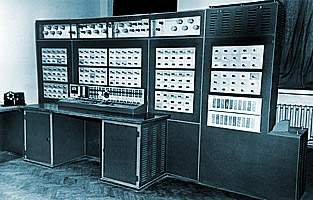
\includegraphics[width=10cm]{Fig1.jpg}
\caption*{1959年时的“Сетунь”,来自\url{http://www.wyzxwk.com/Article/lishi/2011/09/254852.html}}
\end{figure}

(\textit{以上部分道听途说消息并非重点,请勿太过在意})

插播一则智力测试题:
\begin{quote}
你在和小刚玩扑克牌游戏,你的好朋友小明站在小刚身后,不停向你示意他的牌面;假设这副扑克牌不是普通的扑克牌,它的牌面最高有1000,而小明只能用十根手指的屈伸向你传递信息,那么,他如何才能最高效地表示数字?(单次能表示的数字最大)
\end{quote}
但是,二进制有一个大问题,就是其每一位权值相对实在太低,很容易写出一长串数字,人脑难以处理。所以,在实际的逻辑设计中,我们往往还会用到\textbf{16进制}。它与二进制之间的转换比较直观,因此应用广泛:

\begin{figure}
    \begin{tabular}{|c|c|c|c|c|c|}\hline\rowcolor{lightgray}
        十进制 & 二进制 & 十六进制 & 十进制 & 二进制 & 十六进制\\\hline
        0&0000&0&8 &1000&8\\\hline
        1&0001&1&9 &1001&9\\\hline
        2&0010&2&10&1010&A\\\hline
        3&0011&3&11&1011&B\\\hline
        4&0100&4&12&1100&C\\\hline
        5&0101&5&13&1101&D\\\hline
        6&0110&6&14&1110&E\\\hline
        7&0111&7&15&1111&F\\\hline
    \end{tabular}
\end{figure}

注意到,因为懒惰的人类只定义了十个数字,所以当进制超过十时,就会需要从英语字母表“借”字母来表示数字。因此,A=10, B=11, C=12,等等。(至于超过三十六进制后怎么办?我也不晓得)

这样,计算机中最小的处理单位,字节(8bit,一个bit即二进制数的一个数位),就可以表示为一个两位十六进制数,比原先的二进制数串优雅不少。(在电路设计中,有时也会说“该电路接收一个十六进制输入”:这可不是说这个电路能识别3或者9这样的数字,而只是说它以四位bit为一组表示数据)

\begin{figure}
    \begin{tabular}{|>{\columncolor{lightgray}}c|c|c|c|c|c|c|c|c|c|c|}\hline\rowcolor{lightgray}
        \cellcolor{white}$\times$ & 0 & 1 & 2 & 3 & 4 & 5 & 6 & 7 & 8 & 9\\\hline
        0 & 00 & 00 & 00 & 00 & 00 & 00 & 00 & 00 & 00 & 00\\\hline
        1 & 00 & 01 & 02 & 03 & 04 & 05 & 06 & 07 & 08 & 09\\\hline
        2 & 00 & 02 & 04 & 06 & 08 & 0A & 0C & 0E & 10 & 12\\\hline
        3 & 00 & 03 & 06 & 09 & 0C & 0F & 12 & 15 & 18 & 1B\\\hline
        4 & 00 & 04 & 08 & 0C & 10 & 14 & 18 & 1C & 20 & 24\\\hline
        5 & 00 & 05 & 0A & 0F & 14 & 19 & 1E & 23 & 28 & 2D\\\hline
        6 & 00 & 06 & 0C & 12 & 18 & 1E & 24 & 2A & 30 & 36\\\hline
        7 & 00 & 07 & 0E & 15 & 1C & 23 & 2A & 31 & 38 & 3F\\\hline
        8 & 00 & 08 & 10 & 18 & 20 & 28 & 30 & 38 & 40 & 48\\\hline
        9 & 00 & 09 & 12 & 1B & 24 & 2D & 36 & 3F & 48 & 51\\\hline
    \end{tabular}
    \caption*{十六进制下的九九乘法表,是否有一种别样的简洁之美?(并没有)}
\end{figure}
用数学一点的定义,对于$n$进制表示的$m$位整数$(\overline{d_{m-1}d_{m-2}...d_0})_n,\,d\in\mathbb{Z}_n$,每一位都有一个确定的权值,因此可以用位权展开式表示为:$\displaystyle\sum_{i=0}^md_i\cdot n^i$;比如,十进制数$19163=1\times10^4+9\times10^3+1\times10^2+6\times10^1+3\times10^0$;再比如,二进制数$(11001)_2=1\times2^4+1\times2^3+0\times2^2+0\times2^1+1\times2^0$,也就是25。这样,我们只需解一个方程,就一定可以完成进制的转换。(至于更简单的方法,可以在这里了解:\href{https://baijiahao.baidu.com/s?id=1621423277747819472\&wfr=spider\&for=pc}{6、计算机进制之二进制、十进制、十六进制之间的转换})

\section*{二、编码}
什么是编码?简单地说,就是把信息从一种形式转为另一种——所以,学校的学号是对学生的编码;车牌号是对汽车的编码;编程时程序语言转为机器码也是编码。之前提到,计算机中所有信息都是用0和1来表示的;那么,如何把实际生活中形形色色的信息编码为二进制数就是一个值得研究的问题。

\subsection*{1、十进制数的编码}
首先看看正整数。十进制数转为0与1表示的数——第一反应基本都会是转为二进制表达;除此之外,我们再介绍两种常用编码。

第一种是\textbf{BCD码}。对于163这样的数字,如果没有运算的需求,把它不停模二取余转为二进制实在太浪费运算资源了;因此,就有了折中方案:把十进制下每一位都分别用0/1组合编码。这就是二-十进制码,即BCD码。

实际上,一串0与1的组合只是一个符号,本身不需携带太多意义,随意排列组合出十种编码,再与0到9一一对应就可以了——所以理论上,0到9用4bit编码,可以有$A_{16}^{10}=\dfrac{16!}{6!}=2905943040$种组合。但是,其中有用处的其实并不多。

\begin{itemize}
\item 8421码,即把0到9转为对应的二进制数,因其四位权值分别为8,4,2,1得名。
\item 5421码,四位权值分别为5,4,2,1,表示数据时最高位0,1出现频率相当,有美学意义。
\item 2421码,四位权值分别为2,4,2,1,其中0101~1010不使用。因为权值之和为9,当把数按位取反后与原数之和为9(对9互补),适用于某些运算。
\item 5211码,5421与2421的合体产物。
\item 余三码,把8421码加上0011后得到,可以模拟十六进制运算的进位:考虑计算9+3,即1001+0011。用普通二进制加法,得到1100,并无进位产生,必须要再与1010作比较才能知道有没有进位;而用余三码,实际计算的是12+6,即1100+0110,得到(1)0010,即是8421码下的12。只是要注意,当没有进位时,要把和减去6。
\end{itemize}

\begin{figure}
    \begin{tabular}{|c|c|c|c|c|c|}\hline\rowcolor{lightgray}
        十进制 & 8421 & 5421 & 2421 & 5211 & 余三码\\\hline
        0&0000&0000&0000&0000&0011\\\hline
        1&0001&0001&0001&0001&0100\\\hline
        2&0010&0010&0010&0011&0101\\\hline
        3&0011&0011&0011&0101&0110\\\hline
        4&0100&0100&0100&0111&0111\\\hline
        5&0101&1000&1011&1000&1000\\\hline
        6&0110&1001&1100&1010&1001\\\hline
        7&0111&1010&1101&1100&1010\\\hline
        8&1000&1011&1110&1110&1011\\\hline
        9&1001&1100&1111&1111&1100\\\hline
    \end{tabular}
    \caption*{各类BCD码转换表}
\end{figure}

第二种是\textbf{格雷码},或循环码。它表示的数值+1时,只会改变循环码的一个数位,而不像二进制码下因进位而改变若干数位:比如从7到8,二进制码要同时改变四位,而格雷码只会变一位。

\begin{figure}
    \begin{tabular}{|c|c|c|c|}\hline\rowcolor{lightgray}
        十进制 & 格雷码 & 十进制 & 格雷码\\\hline
        0&0000&8 &1100\\\hline
        1&0001&9 &1101\\\hline
        2&0011&10&1111\\\hline
        3&0010&11&1110\\\hline
        4&0110&12&1010\\\hline
        5&0111&13&1011\\\hline
        6&0101&14&1001\\\hline
        7&0100&15&1000\\\hline
    \end{tabular}
    \caption*{格雷码转换表}
\end{figure}
格雷码的转换原则如下:

\begin{enumerate}
\item 1位格雷码有两个码字
\item $(n+1)$位格雷码中的前$2n$个码字等于$n$位格雷码的码字,按顺序书写,加前缀0
\item $(n+1)$位格雷码中的后$2n$个码字等于$n$位格雷码的码字,按逆序书写,加前缀1
\item $(n+1)$位格雷码的集合=$n$位格雷码集合(顺序)加前缀0+$n$位格雷码集合(逆序)加前缀1\cite{3}
\end{enumerate}

观察格雷码各位数字变化规律:01 10 01 10 01 10 01 10,0011 1100 0011 1100,00001111 11110000,00000000 11111111...也可以推出格雷码数表。而在几章之后,还有一种更直观的推导方式。

\begin{quote}
再插播一则智力题:
相信前一道题,不少人可以想到用二进制表示,每个手指表示一个数位;那我们改变一个场景,小刚发现你和小明的阴谋后,让小明做苦力,给你们记录玩的游戏回合数。限制是,游戏可能有几百轮,但小明仍然只能用十根手指。问题是,小明每次都要屈伸不止一根手指,有时速度过快都反应不过来。有没有更好的编码策略?
\end{quote}

总结一下,有三种最重要的数字编码方案:二进制码,计算优势较大;BCD码,计算效率与直观性的妥协;格雷码,适用于计数。

\divider

在不创造“-”(负号)或者“ . ”(小数点)这样的新符号的前提下,如何表示负数和小数呢?

先来看负数。第一反应自然是在二进制数前多加一位符号位,0为正,1为负:
\[\underbrace{d_{\mathrm{sign}}}_{符号位}\underbrace{\overline{d_{m-1}d_{m-2}...d_0}}_{数字位}\]

所以5变成了0101;-5就是1101。但是设想一个能够实现二进制加法的加法器,让它做13-2的运算:0 1101+1 0010,会得到-15。这是因为,当送入加法器的数是一正一负时,要改变运算法则,变逢二进一为逢零借一,这就需要用到另一组逻辑,显然不是最优解;有没有能统一逻辑的更好的方法?

想象场景:电子表没电了,需要调准时间。手表显示12:56;实际时间12:15,那么,除了把时间往回调41分钟,作为懒惰的人类,还有没有其他方法?稍微思考一下,我们其实还可以向前调19分钟——因为调分钟时忽略小时数的变化,从12:59再向前调一分钟,就又变回了12:00。这就是六十进制下,加减法的转换:因为$x-19\equiv x+41\pmod{60}$,通过忽略进位借位问题,我们把-41转化为了+19。

举一反三,二进制中,$x\equiv x+2^n\pmod{2}$,所以当我们忽略$n$位以上的位数后,就有了$x-m=x+(2^n-m)$,从而把负数$-m$变为了$2^n-m$,其中因为$m$能用$n$位二进制数表示,一定小于$2^n$。我们把$+(2^n-m)$称为$-m$的补码。

回到13-2的问题。因为13和2都能用四位二进制数表示,所以我们取$n=4$,得到-2的补码为16-2=14,即1 1110(符号位是判断究竟表示正还是负的基础,不能变)。然后再做加法运算:0 1101+1 1110=(1)0 1011。舍弃掉进位,就得到了0 1011,即+11。通过补码,成功把减法转化为了加法。既然每次要做关于负数的运算都要有这样的变换,那何不计算时就用补码作为负数的表达形式?(存储时仍可使用直接添加符号位的方法)

\begin{figure}
    \begin{tabular}{|c|c|}\hline\rowcolor{lightgray}
        二进制表示 & 十进制数\\\hline
        0000 0000&$+0$\\\hline
        0000 0001&$+1$\\\hline
           ...   &...\\\hline
        0111 1110&$+126$\\\hline
        0111 1111&$+127$\\\hline
        1000 0000&$-128$\\\hline
        1000 0001&$-127$\\\hline
           ...   &...\\\hline
        1111 1110&$-2$\\\hline
        1111 1111&$-1$\\\hline
    \end{tabular}
    \caption*{用一个字节能表示的所有有符号整数,即编程中的byte类型数据}
\end{figure}

但是,上面得到的这么多数,都是一个个老老实实用128减去原数得到的吗?其实还有一种简单的方法,即先将所有数字位取反——0变1,1变0——再加上1。

为了证明$1000\,0000-\overline{b_7b_6...b_0}=\overline{b_7'b_6'...b_0'}+1$,我们只需注意到,因为$b_n$和$b_n'$永远一个为0,一个为1,所以$\overline{b_7b_6...b_0}+\overline{b_7'b_6'...b_0'}=0111\,1111$。移项,然后等号两边同时+1即可。

解决了负数,再来看小数。

关于小数,最优解是把数用科学记数法表示。 

\[x=a\times k^m,\,a\in[1,2)\]

我们可以先确定$k$的值。十进制科学记数法中,指数每+1,小数点都会左移一位,对应数$\times 10$;二进制下,小数点的左移一位,也是$\times 10$,不过是二进制下的10,实际上是$\times 2$。因此,科学记数法中底数应该选择2,才能达到指数加一,小数点移一位的效果。

\[x=a\times 2^m\]

下一个,$a$与$m$都是参数,位数都不固定(当是无限小数时甚至可以无限大),但这个小数总共能占据的空间是有限的,固定的。当$a$分配的位数比较多,而$m$位数比较少时,可以表示很精确的数,但所能表示的范围较小;相对地,如果$m$位数变多,那么所能表示的范围变大,而精度降低。在这其中,必须要做出妥协。

1985年,IEEE(Institute of Electrical and Electronics Engineers,美国电气和电子工程师协会)首次制定了统一的浮点数(可以简单地理解成“小数点位置可以移动的数”)表示规范,最新的IEEE754-2019规范中,主要有单精度与双精度两种形式,分别占用两个字节和四个字节;一个数又可以分为Sign(符号),exponent(指数)和mantissa(尾数)三部分。具体规范如下(方括号表示比特位):

\begin{figure}
    \begin{tabular}{|c|c|c|c|}
        \multicolumn{4}{c}{Floating Point Components}\\\hline
        &Sign&Exponent&Fraction\\\hline
        Single Precision&1 [31]&8 [30-23]&23 [22-00]\\\hline
        Double Precision&1 [63]&11 [62-52]&52 [51-00]\\\hline
    \end{tabular}
\caption*{来源:\url{https://www.cnblogs.com/german-iris/p/5759557.html},此博客也提供了详细的浮点值处理方法}
\end{figure}

而更详细的浮点数计算、赋值等规范,在此时就不是那么重要了。

至此,我们大概地了解了负数与小数的表示规范。

\subsection*{2、字符的编码}
随着计算机交互的兴起,如何传递文字也成了亟待解决的问题。于是,60年代,美国率先制定了以拉丁字母为基础的ASCII(美国信息交换标准代码)表——它的理念很简单,只要把常用字符都用二进制表达,然后让双方计算机都认可这一协议规范即可。表格如下:

\begin{figure}
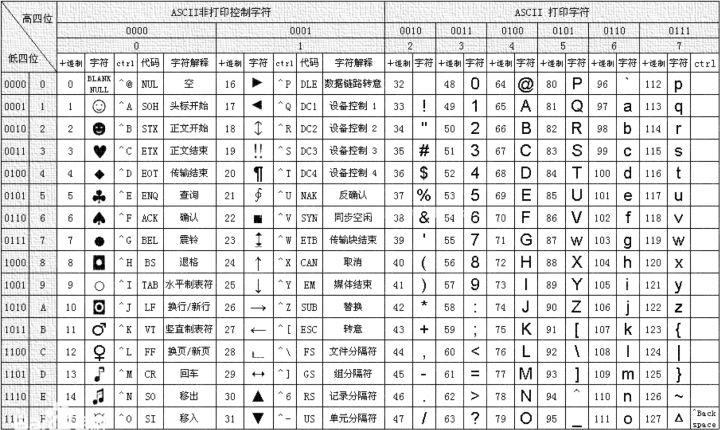
\includegraphics[width=16cm]{Fig2.jpg}
\caption*{来自百度百科ASCII词条,有编辑}
\end{figure}
ASCII使用了一个字节中的七个bit,最高位留空。

其后字符编码的需求愈发扩大,尤其是计算机在亚洲国家逐渐普及,于是Unicode应运而生。它有17个编码集合;每个集合从0000至FFFF共65536个位置可编码。其中ASCII码也是Unicode的一个子集。

除此之外,图像、音频等也有其各自的编码策略,这里不再赘述。

\begin{thebibliography}{5}
\bibitem{1} \url{https://baike.baidu.com/item/三进制计算机/10507483}
\bibitem{2} \url{https://www.jianshu.com/p/059e78199549}
\bibitem{3} \url{https://baike.baidu.com/item/格雷码/6510858?fr=aladdin}
\end{thebibliography}

\end{document}